% don't remove the folling lines, and edit the defintion of \main if needed
\documentclass[../report.tex]{subfiles}
\providecommand{\main}{..}
\IfEq{\jobname}{\currfilebase}{\AtEndDocument{\biblio}}{}
% until here

\begin{document}

%\clearpage

\section{Feebly-interacting particles}
\label{sec:BSM-FIPs}

Unknown particles or interactions are needed to explain a number of observed phenomena and outstanding questions in particle physics, astrophysics and cosmology. While there is a vast landscape of theoretical models that try to address these puzzles, on the experimental side most of the efforts have so far concentrated on the search for new particles with sizeable couplings to SM particles and masses above the EW scale.
An alternative possibility, largely unexplored, is that particles responsible for the still unexplained phenomena are below the EW scale and have not been detected because they interact too feebly with SM particles. 
These particles would belong to an entirely new sector, the so-called {\it hidden} or {\it dark sector}. While masses and interactions of particles in the dark sector are largely unknown, the mass range between the MeV and tens of GeV appears particularly interesting, both theoretically and experimentally, and is the subject of this section.

An important motivation for new physics in this mass range is DM (see Chapter~\ref{chap:dm}), which could be made of light particles, with either a thermal or non-thermal cosmological origin. Thermal DM in the MeV--GeV range with SM interactions is overproduced in the early universe and therefore viable scenarios require additional SM neutral mediators to deplete the overabundance~\cite{Lee:1977ua,Boehm:2002yz,Boehm:2003hm,Pospelov:2007mp,Feng:2008ya,ArkaniHamed:2008qn}. 
These mediators, which must be singlets under the SM
gauge symmetry, can lead to couplings of {\it feebly-interacting particles} to the SM through {\it portal} operators.

%-----------------------------------------------
\subsection{The formalism of portals }
\label{ssec:fips_portals}
%-----------------------------------------------

Portals are the lowest canonical-dimension operators that mix new dark-sector states with gauge-invariant (but not necessarily Lorentz-invariant) combinations of SM fields. Following closely the scheme used in the Physics Beyond Colliders study~\cite{Beacham:2019nyx}, four types of portals are considered:
\begin{center}
\begin{tabular}{c|l}
Portal & Coupling \\
 \hline
Vector (Dark Photon, $A_{\mu}$) &  $-\frac{\epsilon}{2 \cos\theta_W} F^\prime_{\mu\nu} B^{\mu\nu}$ \\ 
Scalar (Dark Higgs, $S$) & $(\mu S + \lambda_{HS} S^2) H^{\dagger} H$  \\ 
Fermion (Sterile Neutrino, $N$) & $y_N L H N$ \\ 
Pseudo-scalar (Axion, $a$) &  $\frac{a}{f_a} F_{\mu\nu}  \tilde{F}^{\mu\nu}$, $\frac{a}{f_a} G_{i, \mu\nu}  \tilde{G}^{\mu\nu}_{i}$,
$\frac{\partial_{\mu} a}{f_a }\overline{\psi} \gamma^{\mu} \gamma^5 \psi$
\end{tabular}
\end{center}
Here $F^\prime_{\mu \nu}$ is the field strength for the {\it dark photon}, which mixes with the hypercharge field strength
$B^{\mu\nu}$; $S$ is the {\it dark Higgs}, a new scalar singlet that couples to the SM Higgs doublet
$H$;
and $N$ is a {\it heavy neutral lepton} (HNL)
that couples to the SM left-handed leptons. These three cases are the only possible renormalisable portal interactions. While many new operators can be written at the non-renormalisable level, a particularly important example is provided by the {\it axion} (or axion-like) particle $a$ that couples to gauge and fermion fields at dimension five.

%-----------------------------------------
\subsection{Experimental sensitivities}
\label{ssec:fips_sensitivities}
%-----------------------------------------
The portal framework is used to define some benchmark cases, for which sensitivities of different experimental proposals are evaluated and compared with each other. 
Unless otherwise stated, all limits presented in this section correspond to 90\% CL, since the majority of the literature has been using this standard.

\noindent
%---------------------------
{\bf Vector portal} \\
%---------------------------    
New light vector particles mixed with the photon are not uncommon in BSM models containing hidden sectors, possibly related to the DM problem.
The parameters describing this class of models are $\epsilon$, $\alpha_D$, $m_{A'}$ and $m_{\chi}$,
where $\epsilon$ is the mixing parameter between the dark and ordinary photon; $\alpha_D = g^2_D/ 4 \pi$ is the coupling strength of the dark photon with DM; and $m_{A^\prime}$ and $m_{\chi}$ are the dark photon and DM particle mass, respectively.
The study of experimental sensitivities at future colliders is performed in the plane of $\epsilon$ versus $m_{A^\prime}$,
assuming $\alpha_D$ to be negligible with respect to $\epsilon$.
It is important to note that only minimal Dark Photon models have been considered in this study. 
Non-minimal models used by, e.g.\ the \HLLHC experiments~\cite{CidVidal:2018eel} and other future facilities, are not addressed here.
The results are shown in Fig.~\ref{fig:FIPs-DarkPhoton}.
The low-mass range (0.01--1 GeV, see Chapter~\ref{chap:dm}) is best covered by beam-dump experiments (SHiP~\cite{Anelli:2015pba}, NA62 in dump mode~\cite{Lanfranchi:2018xrz}), and by FASER at the ATLAS interaction point~\cite{Ariga:2018pin} in the very low-coupling regime ($\epsilon < 10^{-4}$). These are complemented by the LHCb Upgrade~\cite{Ilten:2015hya} and Belle-II~\cite{Kou:2018nap}. Future collider experiments (HL-LHC~\cite{Curtin:2014cca}, \CEPC~\cite{CEPCStudyGroup:2018ghi}, \FCCee~\cite{Karliner:2015tga}, \FCChh~\cite{Curtin:2014cca}, {\ILCFiveHundred}) have unique coverage in the high-mass range ($>$ 10 GeV) down to $\epsilon \sim 10^{-4}$.  \FCCeh 
%[ref Fisher, private communication] 
could fill the gap left by LHCb in the low-mass region. There is an interesting complementarity between future collider experiments, which cover the high-mass large-coupling regime, and beam-dump experiments, which cover the low-mass, very low-coupling regime.

\begin{figure}[htb]
%\begin{figure}[t]
    \centering
    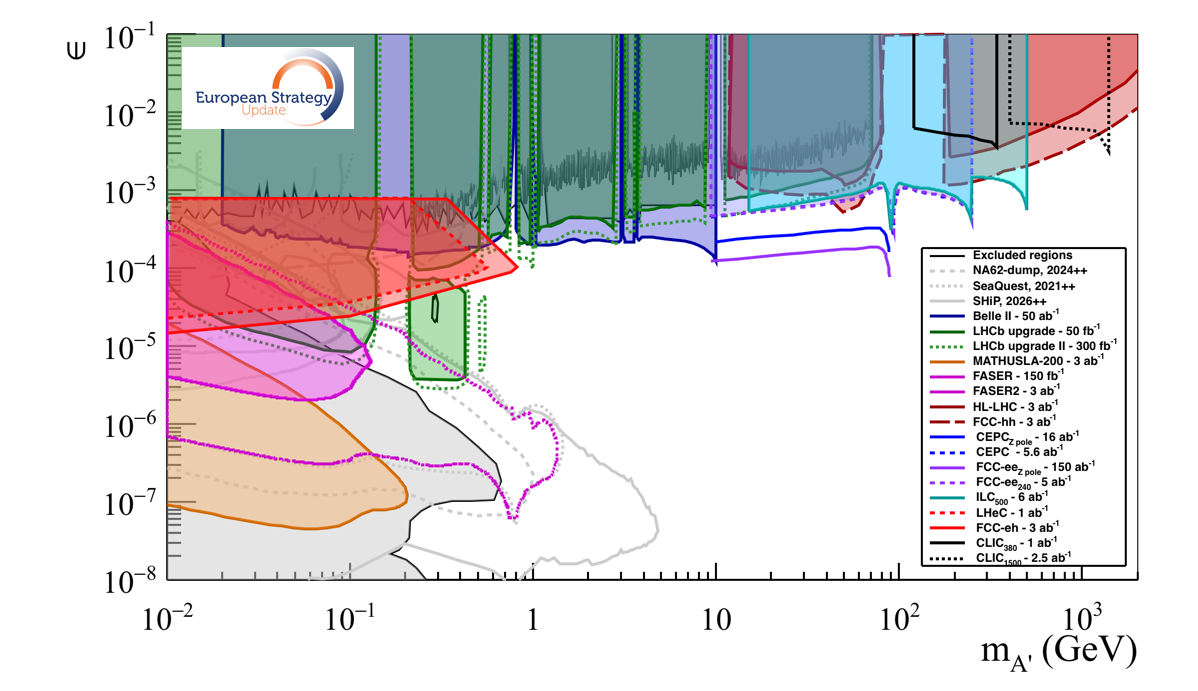
\includegraphics[width=\textwidth]{\main/BSM/FIPs/DP_all.png}
    \caption{Sensitivity for Dark Photons in the plane mixing parameter $\epsilon$ versus Dark Photon mass. HL-LHC, CEPC, FCC-ee and FCC-hh curves correspond to 95\% CL exclusion limits, LHeC and FCC-eh curves correspond to the observation of 10 signal events, and all other curves are expressed as 90\% CL exclusion limits. The sensitivity of future colliders, mostly covers the large-mass, large-coupling range, and is fully complementary to the the low-mass, very low-coupling regime where beam-dump and fixed-target experiments are most sensitive.
    }
    \label{fig:FIPs-DarkPhoton}
\end{figure}


\vskip 2mm
\noindent
%---------------------------
    {\bf Scalar portal} \\
%---------------------------
In the {\it scalar} or {\it Higgs portal}, the dark sector is coupled to the Higgs boson via the bilinear $H^{\dagger} H$ operator of the SM. The minimal scalar portal model operates with one extra
singlet field $S$ and two types of couplings, $\mu$ (or $\sin \theta$)  and $\lambda_{HS}$~\cite{OConnell:2006rsp}. 
The coupling constant $\lambda_{HS}$ leads to pair-production of $S$ but cannot induce its decay, which requires a non-vanishing $\sin \theta$.
This portal has several theoretical motivations. The new scalar can generate the baryon asymmetry of the universe~\cite{Cohen:1987vi} and play the role of mediator
between SM particles and light DM in case of secluded annihilations ($\chi \chi \to \phi \phi$, where $\chi$ is the light DM particle and $\phi$ the light scalar mediator) ~\cite{Krnjaic:2015mbs}.
It can also address the Higgs fine-tuning problem (via the {\it relaxion} mechanism ~\cite{Graham:2015cka}), which generically leads to relaxion-Higgs mixing~\cite{Flacke:2016szy} 
and provides an alternative baryogenesis mechanism~\cite{Abel:2018fqg} and a DM candidate~\cite{Fonseca:2018xzp,Banerjee:2018xmn}. 

The experimental sensitivities are shown in Fig.~\ref{fig:FIPs-DarkHiggs}.
Shaded grey areas are already excluded, as detailed in ref.~\cite{Beacham:2019nyx}.
The low-mass ($< 10$ GeV, see Chapter~\ref{chap:dm}), low-coupling range is optimally covered by SHiP at the Beam Dump Facility and MATHUSLA200. FASER, with 3~ab$^{-1}$ is also sensitive to the same mass range, while CODEX-b and MATHUSLA200 have a unique reach in the high-mass and very low-coupling regime. Vertical lines correspond to the bounds on the Higgs/dark-Higgs quartic coupling $\lambda_{HS}$ and on $m^2_S/v^2$ from the projections for the untagged-Higgs at future colliders~\cite{deBlas:2019rxi} (see discussion in~\cite{Frugiuele:2018coc}). The mass range above a few GeV can be explored also by CLIC and LHeC/FCC-eh using the displaced-vertex technique. The large-coupling regime is covered by $e^+ e^-$ colliders using the recoil technique ($e^+ e^- \to Z S$) or running at the $Z$-pole, via the process $e^+ e^- \to Z \to S \ell^+ \ell^-$.

\begin{figure}[htb]
%\begin{figure}[t]
    \centering
    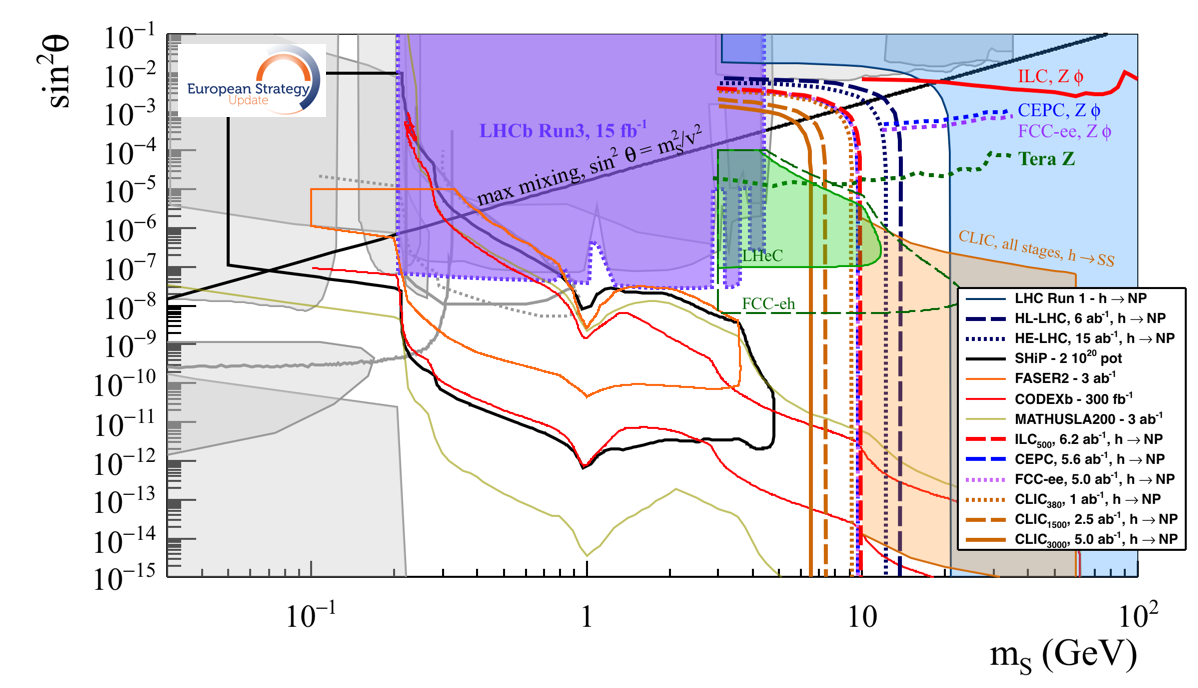
\includegraphics[width=\textwidth]{\main/BSM/FIPs/DS_all.png}
    \caption{Exclusion limits for a Dark Scalar mixing with the Higgs boson. LHeC, FCC-eh, CLIC (all stages) curves and the vertical lines correspond to 95\% CL exclusion limits, while all others to 90\% CL exclusion limits. See text for details.
    }
    \label{fig:FIPs-DarkHiggs}
\end{figure}

\vskip 2mm
\noindent
In the limit of small mixing angle, one can bound the Higgs/dark-Higgs quartic coupling $\lambda_{HS}$ via the Higgs invisible width, which is naturally expected to satisfy the relation $\lambda_{HS}\lesssim m_S^2/v^2$. 
In Table~\ref{table:scalarInv} projections for the constraints on $\lambda_{HS}$ and the scalar mass for various future collider options are provided. 

\begin{table}[h!]
\caption{\small Bounds on the Higgs/dark-Higgs quartic coupling $\lambda_{HS}$, and on the scalar mass $m_S$. The projection for the Higgs invisible width are taken from~\cite{deBlas:2019rxi}.}
\begin{center}
 \begin{tabular}{|c| c c c c c c c c|} 
 \hline
 %\begin{small}
  Collider &{\small HL-LHC} & {\small HL-LHC}& {\small HL-LHC} &  {\small ILC$_{500}$}& {\small  CLIC$_{3000}$}&{\small CEPC} & {\small FCC} & {\small FCC} \\
   & &  {\small + LHeC} &  {\small + HE-LHC} & & & & {\small ee} & {\small ee/eh/hh}
 %\end{small}
 \\ [0.5ex] 
 \hline\hline
 ${\lambda_{HS}/{10^{-3}}}$ & 2.0& 1.5& 1.8& 0.69& 1.2& 0.77& 0.64& 0.23 \\ 
 \hline
$m_S\,$[GeV] & 11& 9.7& 10& 6.5& 8.4& 6.8& 6.2& 3.7\\
 \hline

\end{tabular}
\end{center}
\label{table:scalarInv}
\end{table}
%
\vskip 2mm
\noindent
%--------------------------------
{\bf Pseudo-Scalar portal} \\
%--------------------------------
QCD axions are a central idea in particle physics 
to solve the strong CP problem (see Sect.~\ref{Ref-TBD}).
Current QCD axion models are restricted to the sub-eV mass range. Less constrained are generalisations to axion-like particles (ALPs)~\cite{Jaeckel:2010ni}, which can act as
mediators between light DM and SM particles.
Figure~\ref{fig:FIPs-ALP} shows the sensitivity of future collider experiments to ALPs interacting with photons. 

The typical production mechanisms are: the Primakoff effect and $\pi^0$/$\eta$ decays (see Sect.~\ref{Ref-TBD}) in beam-dump experiments; DY production followed by $Z \to a \gamma$ for hadron colliders; $e^+ e^-  \to (Z) \to a \gamma$ with $a \to \gamma \gamma$ for lepton colliders.
Three mass regions can be clearly identified. The region $m_a < 1$~GeV is dominated by beam-dump experiments in the very low-coupling regime and by FASER2~\cite{Ariga:2018pin}. In this mass regime, ALPs have a lifetime long enough to escape direct detection in experiments at future colliders, and can be identified only via missing energy.
The intermediate mass region (1~GeV $< m_a < $ 90~GeV) can be optimally explored by $e^+ e^-$ colliders (\CEPC~\cite{CEPCStudyGroup:2018ghi}, \CLIC~\cite{deBlas:2019rxi}, \ILC, 
%[peskin, private communication], 
\FCCee~\cite{Bauer:2018uxu}) running at the $Z$-pole and by hadron colliders (\FCChh~\cite{Bauer:2018uxu}) via $Z$ decays). In most of this mass range, the two photons from $a$ decays are not resolved and, hence, the ALP mass cannot be determined. Finally the high-mass region (from tens of GeV to a few TeV) can be optimally explored  by $e^+ e^-$ linear colliders (\ILC and \CLIC) and $ep$ colliders (LHeC and \FCCeh~\cite{Yue:2019gbh}).
Future collider experiments can also search for ALPs with fermion and gluon couplings but the corresponding sensitivity curves have been evaluated only in a few cases and are not considered in this study. 

%\begin{figure}[t]
\begin{figure}[htb]
    \centering
    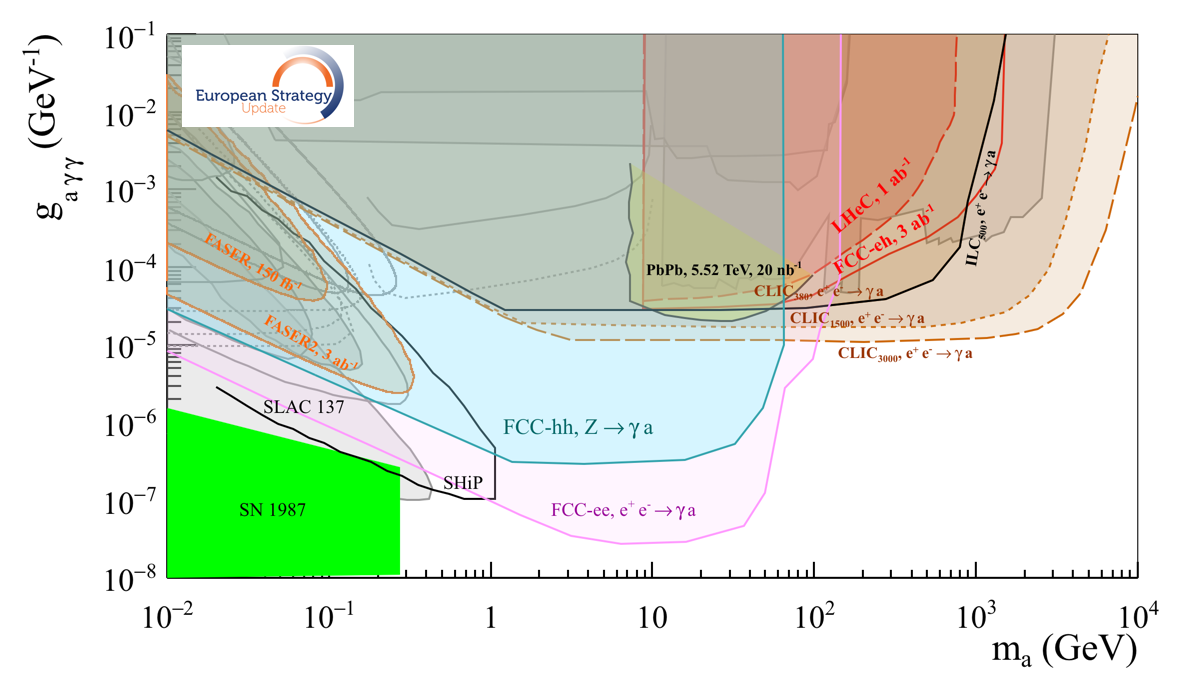
\includegraphics[width=\textwidth]{\main/BSM/FIPs/ALPS_gg_all.png}
    \caption{Exclusion limits for ALPs coupled to photons. All curves correspond to 90\% CL exclusion limits, except for LHeC/FCC-eh (95\% CL exclusion limits), FCC-ee (observation of four signal events) and FCC-hh (observation of 100 signal events). See text for details.}
    \label{fig:FIPs-ALP}
\end{figure}

\vskip 2mm
\noindent
%--------------------------
{\bf Fermion portal} \\
%---------------------------
%The existence of right-handed neutrinos $\nu_R$ or {\it Heavy Neutral Leptons} (HNL) is an open question with important consequences that range from the origin of neutrino masses to the leptogenesis mechanism as an explanation for the cosmic baryon asymmetry (see Sect.~\ref{Ref-TBD}). The scale of HNL masses is entirely unknown and different choices can have a wide range of implications for particle physics, astrophysics and cosmology (for an overview see e.g. \cite{Drewes:2013gca}). In the Neutrino Minimal Standard Model ($\nu MSM$)~\cite{Asaka:2005pn} two HNLs are expected to be in the range MeV--GeV, while a third HNL is a DM candidate with mass as low as a few keV. 
The physics case for {\it Heavy Neutral Leptons} (HNL) is discussed in Chapter~\ref{chap:neut} and here only a summary of projections on the experimental reach is presented.

Figure~\ref{fig:FIPs-HNL} shows the sensitivity of experiments at current and future accelerators to the mixing parameter between the electron neutrino and HNL
in the mass range 0.1--100 GeV. The low-mass range ($< 5$ GeV) is dominated by SHiP at the Beam Dump Facility, followed by experiments at the LHC interaction points, MATHUSLA200, FASER, CODEX-b~\cite{Beacham:2019nyx}. The mass region between 5 and about 90 GeV can be explored by \ILC~\cite{Antusch:2017pkq}, \CEPC~\cite{CEPCStudyGroup:2018ghi} and \FCCeh~\cite{Abada:2019zxq}, being dominated by the \FCCee running at the $Z$-pole~\cite{Abada:2019zxq}.
HNL with masses above 90 GeV can be directly searched for using displaced-vertex techniques at \FCCeh~\cite{Abada:2019zxq} and \FCChh~\cite{Antusch:2016ejd}, and with indirect techniques at \FCCee, \CEPC and \ILC. Among indirect techniques, EW precision measurements allow the sensitivity to HNL to be extended up to very high masses, well beyond what shown in Fig.~\ref{fig:FIPs-HNL}. Finally, SHiP and \FCCee running at the $Z$-pole have the potential to exclude the region of masses and couplings compatible with leptogenesis~\cite{Eijima:2018qke} almost down to the see-saw limit. 

\begin{figure}[htb]
%\begin{figure}[t]
    \centering
    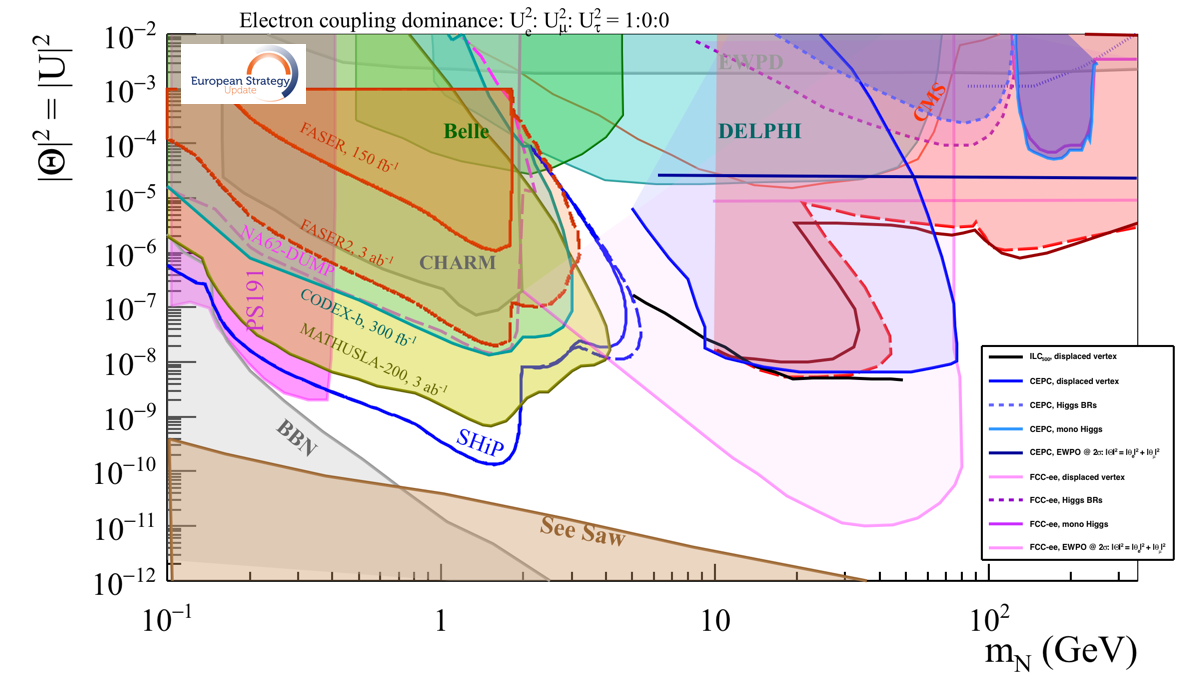
\includegraphics[width=\textwidth]{\main/BSM/FIPs/HNL_Ue_all.png}
    \caption{90\% CL exclusion limits for a Heavy Neutral Lepton mixed with the electron neutrino. See text for details.
    }
    \label{fig:FIPs-HNL}
\end{figure}
%
%\vskip 2mm
%\noindent
%--------------------------------
%{\bf Summary} \\
%--------------------------------
%The absence, so far, of unambiguous signals of new physics from direct searches at the LHC, indirect searches in flavour physics and direct DM detection experiments, along with the absence of a clear guidance from theory about the next scale in nature, necessitates the broadening of the experimental effort in the quest for new physics and in exploring ranges of interaction strengths and masses different from what is already covered by existing or planned initiatives. Feebly-interacting particles represent an alternative paradigm with respect to the traditional BSM physics explored at the LHC. The full investigation of this paradigm over a large range of couplings and masses requires a great variety of experimental facilities. In this context, the physics reach of experiments at future colliders is complemented by beam-dump facilities which typically cover the range of low masses and extremely feeble couplings. 

\end{document}

